\chapter{Methodology}
% This chapter is for going over my methods and talking about my software architecute and why it looks the way it does.

\section{Research Design} 
\paragraph{}
This thesis is a mixture of both research and design implementation.
The research portion of this project focused on linking an existing C++ application (CuraEngine) into a larger JavaEE based project.
This research also included running a closed beta test of the software and logging the results.

%Diagram of how the user interacts with WebSlicer from a high level .
\begin{figure}[!ht]
  \centering
  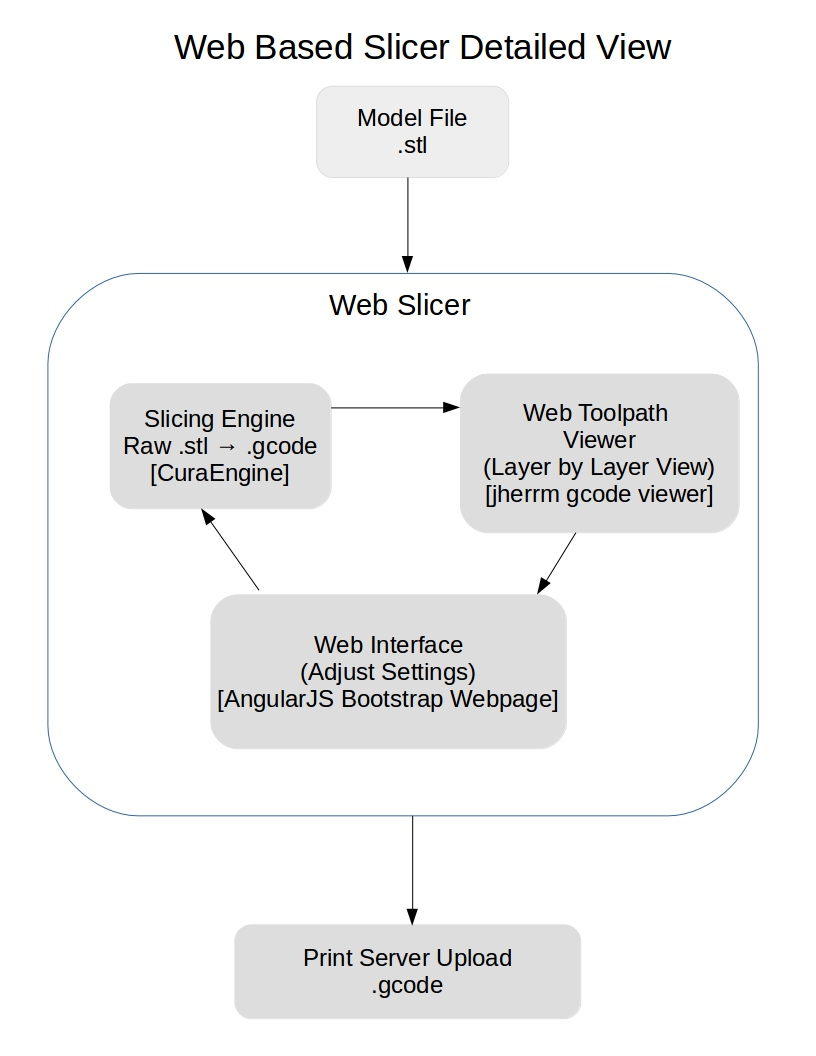
\includegraphics[width=\linewidth]{slicer-detailed-view}
  \caption{High level view of how WebSlicer functions and how users will interact with it}
  \label{fig:slicer-detailed-view}
\end{figure}

\section{Working procedure}
\paragraph{}
% this needs way more info
As shown in Figure \ref{fig:slicer-detailed-view}, the application will have 3 major components that all need to work together in a cycle until the user decides that the output is what they desire.

\subsection{Web Interface}
\paragraph{}
The web interface includes a set of forms for collecting the users settings for their printer and the settings as they relate to printing the model itself.
This interface also includes an interface so that the user may retain the files they have uploaded for future use.
This does not include the actual slicing engine which must be driven and accessed independently.

\subsection{Slicing Engine}
\paragraph{}
The slicing engine is at the heart of this project. 
It will include taking uploaded .stl model files by the user and convert them into raw G-code. 
The engine that carries out the raw geometry calculations is CuraEngine and is written in pure C++.
Thus, this portion of the project will required deploying CuraEngine on a remote server and creating a RESTful API to interface with it.

\subsection{Web Tool Path Viewer}
\paragraph{}
%expand this with more detail
After configuring and generating the G-code representation for a 3D model, there still must be a way to review visually how the slicing engine actually will split up the model.
This is done by loading the resulting gcode from the slicing engine into a web based visualizer.
The user is then able to view each of the layers and the steps involved in creating each one in detail.
From Figure \ref{fig:slicer-detailed-view} this process of changing settings, slicing, and reviewing can happen an arbitrary number of times before the user decides they are satisfied with the result.

\section{Review and Usability Testing}
\paragraph{}
After running through all steps of the working procedure it was then necessary to test WebSlicer by running a small beta test. 
This beta test consisted of a small group of users with varying familiarity with 3D printing to test how easy WebSlicer is to use through a series of simple tasks.
These simple tasks ranged from uploading a file to finding and adjusting the correct setting for a printer.
